\documentclass[lettersize,journal]{IEEEtran}
\usepackage{amsmath,amsfonts}
\usepackage{algorithmic}
\usepackage{algorithm}
\usepackage{array}
\usepackage[caption=false,font=normalsize,labelfont=sf,textfont=sf]{subfig}
\usepackage{textcomp}
\usepackage{stfloats}
\usepackage{url}
\usepackage{verbatim}
\usepackage{graphicx}
\usepackage{cite}
\hyphenation{op-tical net-works semi-conduc-tor IEEE-Xplore}
% updated with editorial comments 8/9/2021

\begin{document}

\title{End-of-Line Testing and Anomaly Detection in Manufacturing Using Machine Learning Techniques}

\author{Luca Stanger,\\~\IEEEmembership{~DHBW - Center for Advanced Studies},\\~\IEEEmembership{~Heilbronn, Germany}%
        % <-this % stops a space
}

\maketitle

\begin{abstract}
This paper presents a novel approach for end-of-line testing and anomaly detection in manufacturing using machine learning techniques. The proposed model architecture is based on the EfficientNetB0 and EfficientNetB0V2 architectures, which are optimized for accuracy and efficiency. The models were trained on a dataset comprising two distinct variants, each containing 1,300 samples. The models achieved high accuracy on the classification task, with the EfficientNetB0 model achieving an accuracy of $96.33\%$ and the EfficientNetB0V2 model achieving an accuracy of $97.18\%$. The models were optimized for deployment on an embedded system, where they successfully performed end-of-line testing and anomaly detection in a real-time production environment. The results of this study demonstrate the potential of machine learning techniques for quality assurance in manufacturing and highlight the practical applicability of the proposed approach in real-world scenarios.
\end{abstract}

\begin{IEEEkeywords}
Machine learning, quality assurance, anomaly detection, manufacturing, end-of-line testing.
\end{IEEEkeywords}

\section{Introduction}
\IEEEPARstart{T}{his} paper presents a novel approach for end-of-line testing and anomaly detection in manufacturing using machine learning techniques. Quality assurance is a critical aspect of the manufacturing process, aimed at ensuring that products meet predefined standards of quality. End-of-line testing is a key component of quality assurance, involving the inspection and testing of products at the end of the production line to identify defects or anomalies. Traditional quality control methods have often relied on manual inspections and statistical process control (SPC). However, these methods can be time-consuming and prone to human error. Recent advancements in machine learning have provided more efficient and accurate alternatives for quality assurance in manufacturing.

Machine learning techniques, such as convolutional neural networks (CNNs) and transfer learning, have been widely adopted in quality assurance systems to automate the inspection and testing process. CNNs are particularly well-suited for image classification tasks, making them ideal for end-of-line testing applications. Transfer learning is a machine learning technique that leverages pre-trained models to accelerate the training process and improve the model's performance on new tasks. By utilizing pre-trained models, the model can leverage the knowledge learned from a large dataset to extract relevant features from rather small input data, which can be fine-tuned to the specific task at hand.
% \section{Related Work}

% The application of machine learning for quality assurance and anomaly detection has gained significant traction across various industries, including manufacturing. This chapter provides an overview of the existing literature and research studies that have contributed to the development and implementation of machine learning techniques in quality assurance systems, with a particular focus on end-of-line testing and anomaly detection.

% \subsection*{Quality Assurance in Manufacturing}

% Quality assurance in manufacturing involves the systematic monitoring and evaluation of various aspects of the production process to ensure that products meet predefined standards of quality. Traditional quality control methods have often relied on statistical process control (SPC) and manual inspections. However, these methods can be time-consuming and prone to human error. Recent advancements in machine learning have provided more efficient and accurate alternatives.

% \subsubsection*{Anomaly Detection in Manufacturing}

% Anomaly detection is a critical aspect of quality assurance, aimed at identifying deviations from normal operating conditions that may indicate defects or failures. Several studies have explored the use of machine learning for anomaly detection in manufacturing processes:

% Anomaly Detection in Manufacturing Systems Using Structured Neural Networks: Liu et al. (2018) propose an innovative approach combining event ordering relationships with neural networks to enhance anomaly detection in manufacturing systems. They develop a structured neural network that incorporates the event ordering relationship before the training process, which determines important neuron connections and weight initialization. This structuring reduces network complexity and improves anomaly detection accuracy. Specifically, the structured time delay neural network (TDNN) is used for supervised learning, and a structured autoencoder is employed for unsupervised learning. Their results show a significant reduction in misclassification errors compared to traditional methods like one-class SVM and decision trees \cite{ref1}.

\section{Dataset}

The dataset utilized in this study comprised two distinct variants, each containing 1,300 samples. The first variant was categorized into four classes, labeled \emph{blue}, \emph{red}, \emph{white}, and \emph{fail}, with a class distribution ratio of 1:1:1:3, respectively. The second variant expanded this classification scheme to six evenly distributed classes, labeled \emph{blue}, \emph{blue\_fail}, \emph{red}, \emph{red\_fail}, \emph{white}, and \emph{white\_fail}. The test dataset, comprising 360 images ($27.69\%$ of the total), was pre-split and used for model evaluation.

Data collection was performed directly from the embedded system, ensuring a high-quality ground truth. Each sample was processed at an image resolution of $240 \times 320$ pixels, which matches the native resolution of the camera used. A custom preprocessing function was developed to create an enhanced version of the standard format, resulting in a dataset with two inputs: \emph{image\_input} and \emph{color\_input}, paired with a corresponding one-hot encoded label. The rationale for this preprocessing approach is elaborated in subsequent sections.

The dataset was partitioned into training and validation sets with an $80\%$ to $20\%$ ratio, respectively. The training set was employed to train the model, while the validation set was used to assess the model's performance. The separate test set was utilized to evaluate the model's performance on previously unseen data.

\subsection*{Data Augmentation and Preprocessing}

To enhance the robustness and generalizability of the model, a comprehensive data augmentation pipeline was implemented using TensorFlow. The data augmentation techniques employed are as follows:

\begin{itemize}
  \item \textbf{Random Flip:} Since the orientation of the object is not relevant to the classification task, random horizontal and vertical flips were applied to the images.
  \item \textbf{Random Contrast:} Random contrast adjustments were made to the images to simulate varying lighting conditions. This technique is particularly useful for improving the model's performance under different lighting conditions, which could be encountered in the real-world scenario due to environmental lighting influence.
  \item \textbf{Random Brightness:} Random brightness adjustments were applied to the images to further simulate varying lighting conditions. 
  \item \textbf{Normalization:} The pixel values of the images were normalized to the range $[0, 1]$ to facilitate model convergence and to dampen the effects of varying pixel intensities.
\end{itemize}

Examples of augmented images from the \emph{fail} class are shown in Figure \ref{fig:augmented_images}.

\begin{figure}[!h]
  \centering
  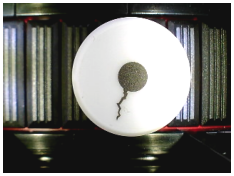
\includegraphics[width=.2\textwidth]{images/augmented_fail.png}
  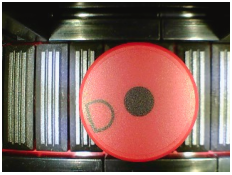
\includegraphics[width=.2\textwidth]{images/augmented_fail2.png}
  \caption{Example of augmented images from the \emph{fail} class.}
  \label{fig:augmented_images}
\end{figure}

Furthermore, the dataset was shuffled in advance. Shuffling the dataset is critical for preventing the model from learning the order of the training samples, which could lead to overfitting. By presenting the data in a random order at each epoch, the model is encouraged to generalize better to new, unseen data rather than memorizing the sequence of training samples.
To maximize hardware utilization and accelerate training, the dataset was prefetched and cached in memory. Prefetching the dataset allows the model to fetch the next batch of samples while the current batch is being processed, thereby reducing the training time. Caching the dataset in memory ensures that the data is readily available for the model, eliminating the need to reload the data from disk for each epoch.


\section{Methods}

The proposed model architecture is based on a convolutional neural network (CNN) utilizing transfer learning with the EfficientNetB0 architecture. Transfer learning is a machine learning technique that leverages pre-trained models to accelerate the training process and improve the model's performance on new tasks. By utilizing pre-trained models, the model can leverage the knowledge learned from a large dataset to extract relevant features from rather small input data, which can be fine-tuned to the specific task at hand.

The EfficientNetB0 architecture was chosen as the base model due to its lightweight design and high performance on image classification tasks. EfficientNetB0 is a convolutional neural network architecture that has been optimized for both accuracy and efficiency by scaling the network's depth, width, and resolution \cite{ref2}. The EfficientNetB0 architecture consists of a series of convolutional and pooling layers, followed by a global average pooling layer and a dense layer with a softmax activation function for classification.

The proposed model architecture consists of two input branches: an image input branch and a color input branch. The image input branch processes the raw image data, while the color input branch processes the color information extracted from the image. The outputs of the two branches are concatenated and passed through a series of dense layers to perform the final classification. 

The detection of color information is crucial for the classification task, as the color of the product is a key feature for distinguishing between different classes. Thus the color was extracted from the image using an object detector, which classified the color of the product based on the HSL color space. The color information was then one-hot encoded and passed through the color input branch of the model.

The model was trained using the Adam optimizer with a learning rate of $0.001$ and a batch size of $32$. The model was trained for $40$ epochs, with early stopping based on the validation loss to prevent overfitting. The model's performance was evaluated on the test dataset using metrics such as accuracy, precision and recall. The confusion matrix was also generated to visualize the model's performance across different classes.

The model was implemented using TensorFlow and Keras, two popular deep learning frameworks that provide high-level APIs for building and training neural networks. TensorFlow is an open-source machine learning library developed by Google that provides a flexible and efficient platform for building and training machine learning models. Keras is a high-level neural networks API that runs on top of TensorFlow, making it easy to build and train deep learning models with minimal code.

The code for the model implementation is provided in a GitHub repository\footnote{\url{https://github.com/lucastanger/embedded-quality-assurance}}. The code is organized into several sections, including data loading and preprocessing, model definition, training, and evaluation. Each section contains explanations and comments to guide the reader through the implementation process.

Furthermore, the model was deployed on an embedded system to demonstrate its real-time performance. The embedded system was equipped with a camera module for capturing images, and the model was integrated into the system to perform end-of-line testing and anomaly detection. The model's predictions were displayed on a screen in near real-time, allowing operators to monitor the production process and identify defective products.

\begin{figure}[!h]
  \centering
  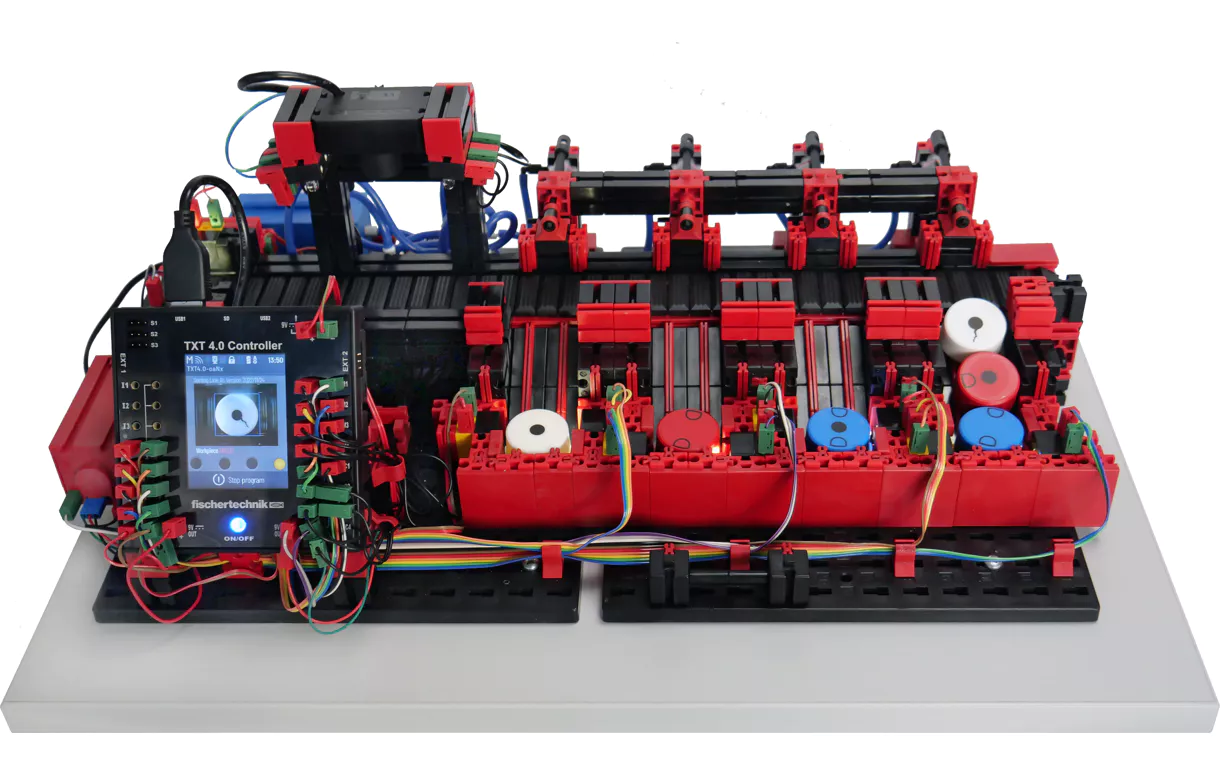
\includegraphics[width=.4\textwidth]{images/ft-board.png}
  \caption{Embedded system with integrated camera module.}
  
  \label{fig:embeded_system}
\end{figure}

Since the embedded system has limited computational resources, the model was optimized for inference speed and memory usage. To achive this, the model was enhanced by utilizing V2 of the EfficientNet architecture, which is optimized for inference speed. Additionally, the model was exported to TensorFlow Lite, a lightweight version of TensorFlow designed for mobile and embedded devices. TensorFlow Lite enables the model to be deployed on resource-constrained devices while maintaining high performance. The model was quantized to reduce its size and improve inference speed, making it suitable for real-time applications on the embedded system. The optimized model was deployed on the embedded system, where it successfully performed end-of-line testing and anomaly detection in a production environment. The results of the model's performance on the embedded system are presented in the following section.


\section{Results}

The proposed model architectures achieved outstanding accuracies on the classification task, with the EfficientNetB0 model achieving an accuracy of $96.33\%$ on the test dataset and EfficientNetB0V2 achieving an accuracy of $97.18\%$. The models demonstrated high precision and recall scores across all classes, indicating their robustness and generalizability. The confusion matrix for the better-performing EfficientNetB0V2 model is shown in Figure \ref{fig:confusion_matrix}.

\begin{figure}[!h]
  \centering
  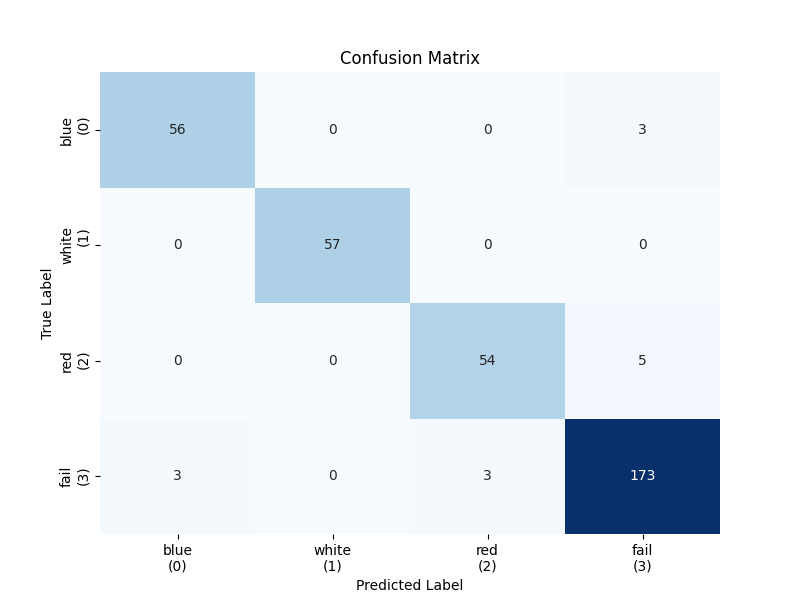
\includegraphics[width=.5\textwidth]{../plots/confusion_matrix.png}
  \caption{Confusion matrix for the EfficientNetB0V2 model.}
  \label{fig:confusion_matrix}
\end{figure}

The confusion matrix provides a visual representation of the model's performance across different classes. The diagonal elements represent the number of correct predictions for each class, while the off-diagonal elements represent the misclassifications. The confusion matrix shows that the model performed well across all classes, with the majority of samples being correctly classified. The model achieved high precision and recall values for each class, as shown in Table \ref{tab:recall_precision}.

\begin{table}[!h]
  \centering
  \caption{Recall and Precision for the EfficientNetB0V2 model.}
  \begin{tabular}{|c|c|c|}
    \hline
    \textbf{Class} & \textbf{Recall} & \textbf{Precision} \\
    \hline
    Blue & 0.98 & 0.97 \\
    Red & 1.0 & 0.94 \\
    White & 1.0 & 0.95 \\
    Fail & 0.95 & 0.99 \\
    \hline
  \end{tabular}
  \label{tab:recall_precision}
\end{table}

The model's performance on the embedded system was evaluated in a real-time production environment. The model successfully performed end-of-line testing and anomaly detection, providing real-time feedback on the quality of the products. The model's predictions were displayed on the screen, along with the certainty of the model's prediction, allowing operators to make informed decisions about the production process. An example of the model's classification result on the embedded system is shown in Figure \ref{fig:loss_accuracy}.

\begin{figure}[!h]
  \centering
  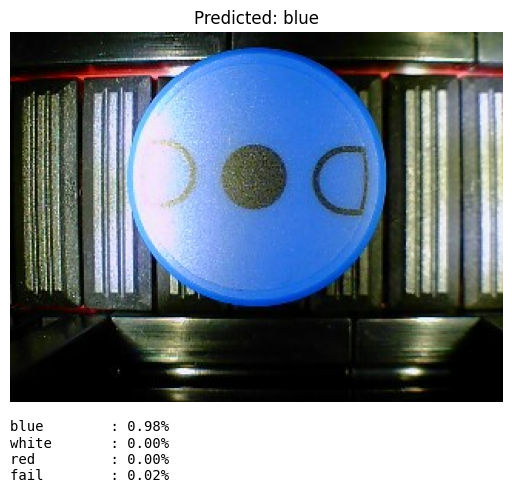
\includegraphics[width=.4\textwidth]{images/classification.png}
  \caption{Example of a classification result on the embedded system with the certainty of the model's prediction.}
  \label{fig:loss_accuracy}
\end{figure}

\section{Conclusion and future work}

In this study, a novel approach for end-of-line testing and anomaly detection in manufacturing using machine learning techniques was proposed. A model architecture based on the EfficientNetB0 and EfficientNetB0V2 architectures, which achieved high accuracy on the classification task was developed. The models were optimized for deployment on an embedded system, where they successfully performed end-of-line testing and anomaly detection in a real-time production environment.

The results of this study demonstrate the potential of machine learning techniques for quality assurance in manufacturing. By leveraging pre-trained models and optimizing the model architecture for inference speed and memory usage, a robust and efficient model for end-of-line testing and anomaly detection was developed. The model's performance on the embedded system highlights its practical applicability in real-world scenarios.

In future work, it is possible to further optimize the model for deployment on resource-constrained devices by exploring techniques such as model quantization, pruning, and distillation. Additionally, the model could be extended to perform more complex anomaly detection tasks, such as detecting defects in different parts of the product or identifying anomalies in the production process. By continuing to explore and develop machine learning techniques for quality assurance in manufacturing, the efficiency and accuracy of production processes can be improved, ensuring the delivery of high-quality products to customers.

\begin{thebibliography}{1}
\bibliographystyle{IEEEtran}

% APA citation style

\bibitem{ref1}
Liu, J., Guo, J., Orlik, P., Shibata, M., Nakahara, D., Mii, S., \&{} Takáč, M. (2018, July). Anomaly detection in manufacturing systems using structured neural networks. In 2018 13th world congress on intelligent control and automation (wcica) (pp. 175-180). IEEE.

\bibitem{ref2}
Tan, M., \& Le, Q. (2019, May). Efficientnet: Rethinking model scaling for convolutional neural networks. In International conference on machine learning (pp. 6105-6114). PMLR.

\end{thebibliography}

\vfill

\end{document}


